\section{Results}

\subsection{Evaluation of Performance}

\begin{figure}[h]
\begin{center}
{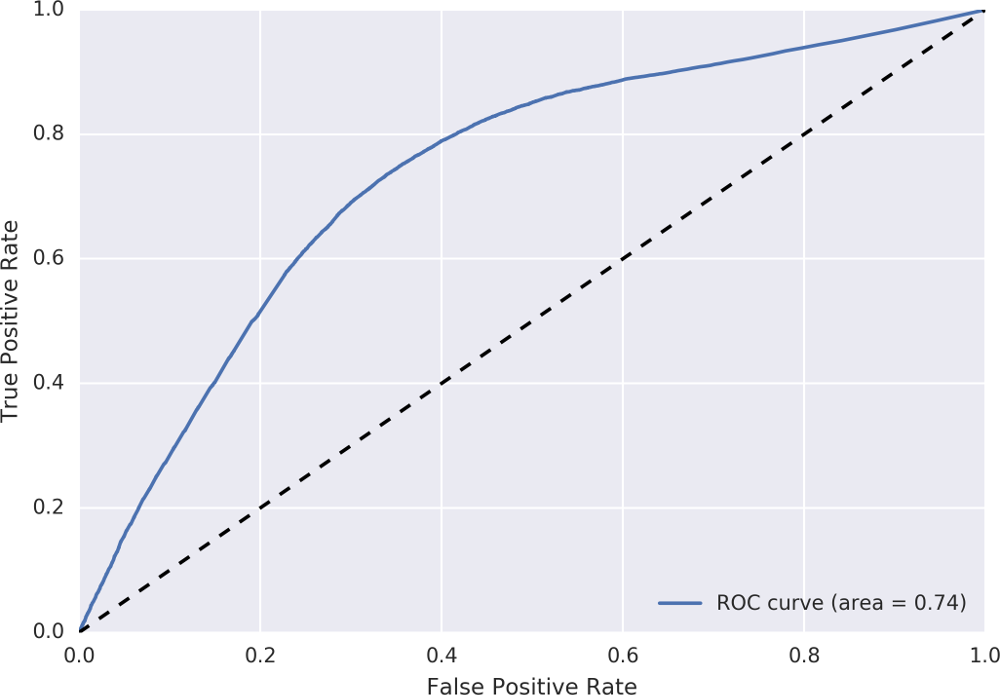
\includegraphics[width=0.9\columnwidth]
{figures/ROC_BETA/ROC_Beta_based_approach_201504.png}}
\caption{ROC curve for prediction procedure. We observed an $\AUC = 0.74$ indicating that our predictor is better than a random predictor ($\AUC \simeq 0.50$).}
\label{ROC_multiclass}
\end{center}
\end{figure}

Alternatively we can evaluate the performance of our model by computing its accuracy for a given threshold $\tau$ of $\FPR$, computed as the ratio between $\TP$ and $\TN$ over the total polulation for a certain $\FPR$. The best accuracy obtained is \num{0.71} for $\tau = 0.4$.
